\chapter{Virtuelle Private Netzwerke}

Der Zugriff aus der Ferne auf das lokale Firmennetzwerk ist für verschiedene Anwendungsszenarien unabdingbar. Die Vernetzung von Firmenstandorten, der Zugriff von mobilen Mitarbeitern auf das Firmennetz oder auch ein Zugang für Geschäftspartner auf das Intranet des Unternehmens müssen sicher Umgesetzt werden.
Die Technologie, die dies ermöglichen soll ist \emph{VPN}. Ein VPN ist ein virtuelles privates Netz, eine logische Verbindung die auf einem anderen, physischen Netz aufgebaut wird \cite{zisler2018computer}. Grundsätzlich eignet sich hier jedes Netz, hier wird jedoch nur die Verwirklichung von VPN über das Internet betrachtet. Es wird zwischen drei Varianten unterschieden:
\begin{itemize}
  \item Site-to-Site/ Branch Office VPN: Verbindung von verschiedenen Firmenstandorten,
  \item End-to-Site/ Remote Access VPN: Verbindung eines Heimarbeitsplatzes oder eines Mobilen Mitarbeiters it dem Intranet des Unternehmens.
  \item End-toEnd VPN: Verbindung zweier Endgeräte,
  \item Extranet VPN: gewährt einem Geschäftspartner/Kunden/Lieferanten Zugang zu Teilen des Internen Netzes 
\end{itemize}


\section{Funktionsweise}





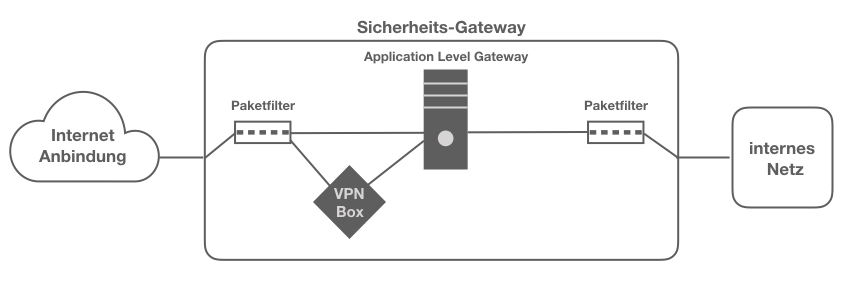
\includegraphics[width=\linewidth]{vpnarchitektur.jpeg}

\section{VPN in privaten Haushalten}